\chapter{Multi-Experiment Supplementary Figures}\label{apdx:gd_spatial_maps}

\begin{figure}[h]
    \centering{
        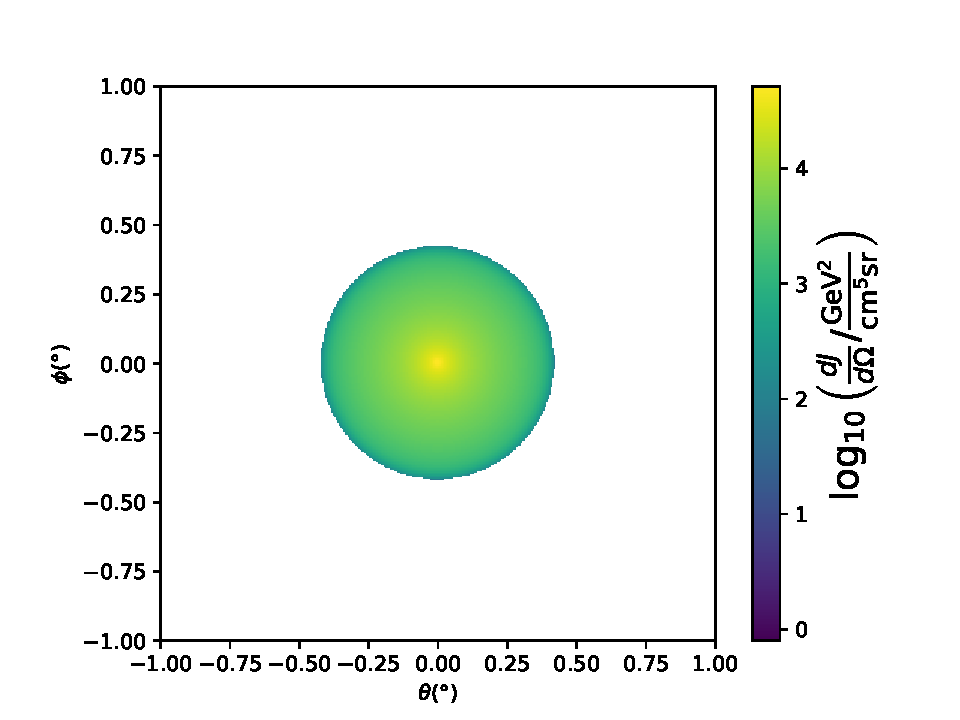
\includegraphics[scale=0.33]{figures/glory_duck/hawc/GD_mass_profiles/BootesI_J_plot.pdf}
        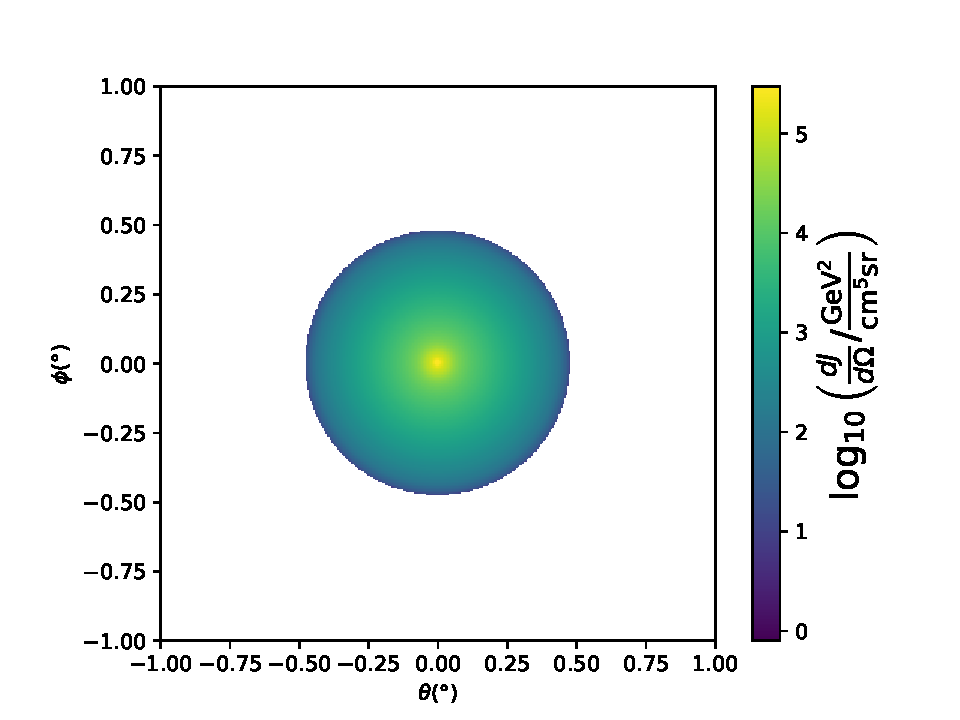
\includegraphics[scale=0.33]{figures/glory_duck/hawc/GD_mass_profiles/CanesVenaticiI_J_plot.pdf}
        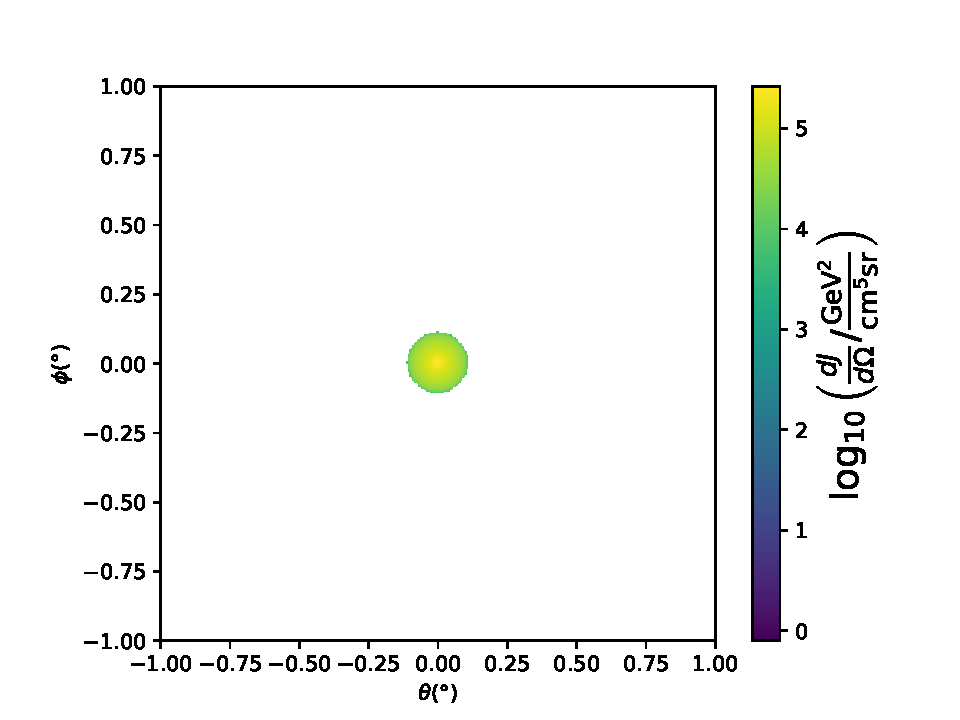
\includegraphics[scale=0.33]{figures/glory_duck/hawc/GD_mass_profiles/CanesVenaticiII_J_plot.pdf}
        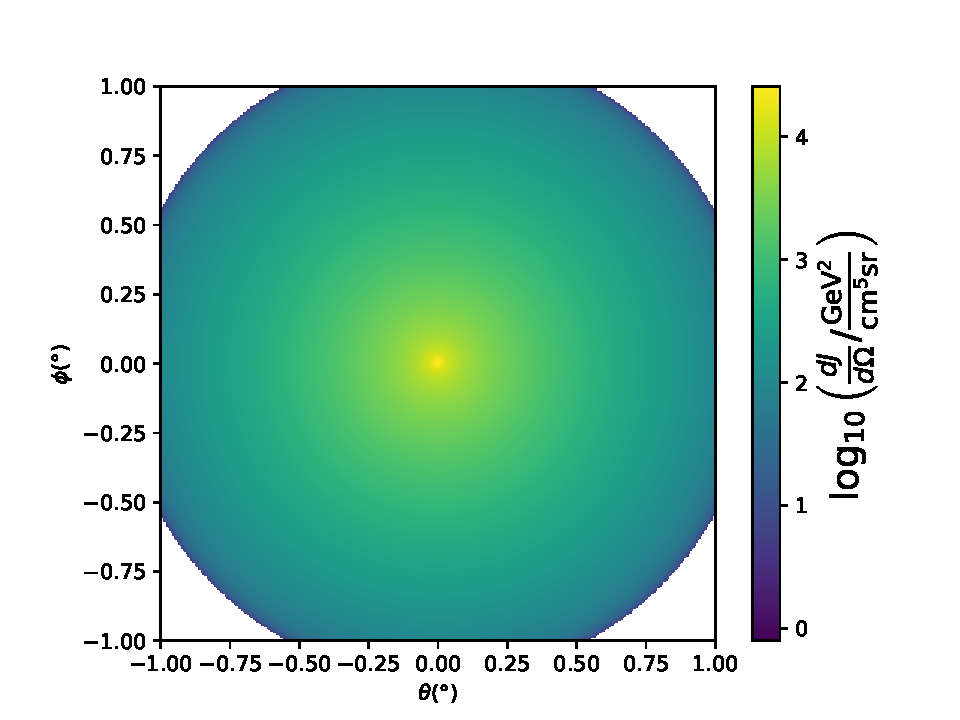
\includegraphics[scale=0.33]{figures/glory_duck/hawc/GD_mass_profiles/Draco_J_plot.pdf}
        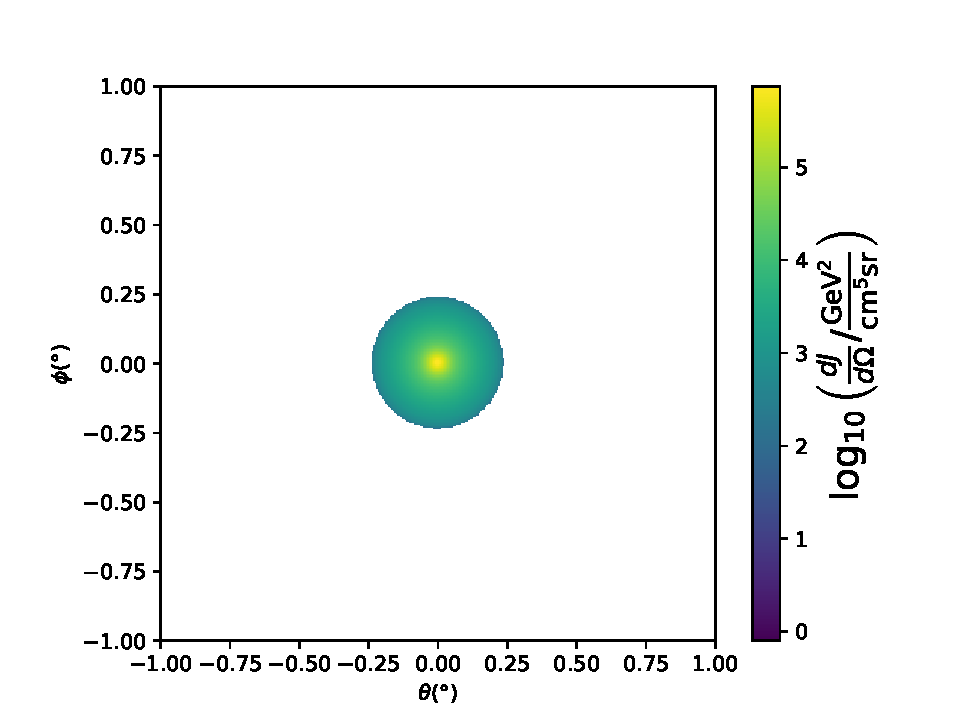
\includegraphics[scale=0.33]{figures/glory_duck/hawc/GD_mass_profiles/Hercules_J_plot.pdf}
        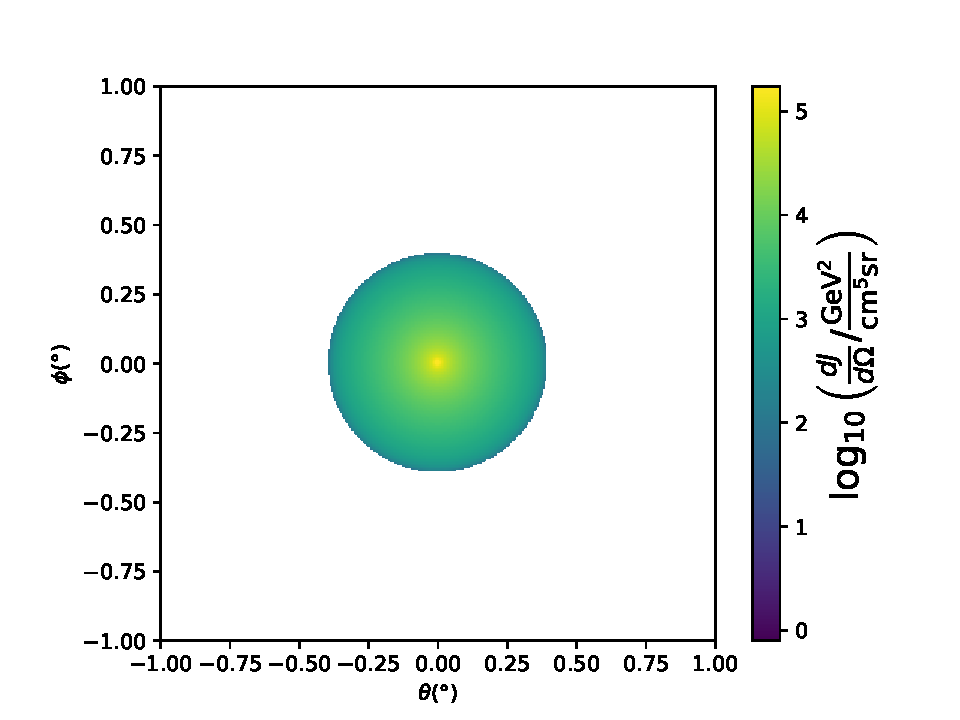
\includegraphics[scale=0.33]{figures/glory_duck/hawc/GD_mass_profiles/LeoI_J_plot.pdf}
        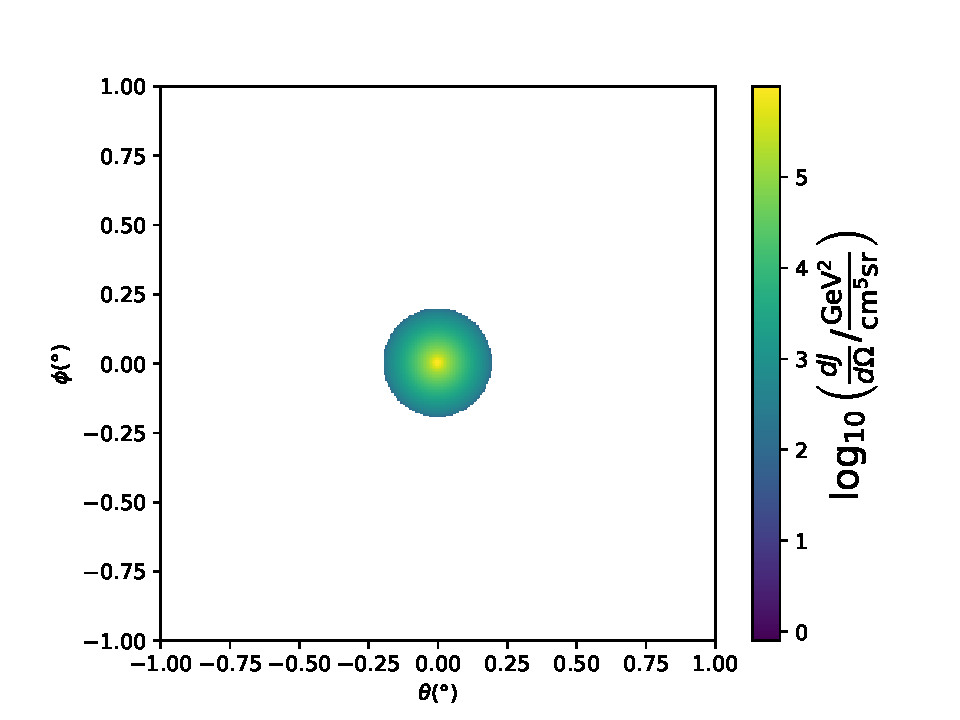
\includegraphics[scale=0.33]{figures/glory_duck/hawc/GD_mass_profiles/LeoII_J_plot.pdf}
        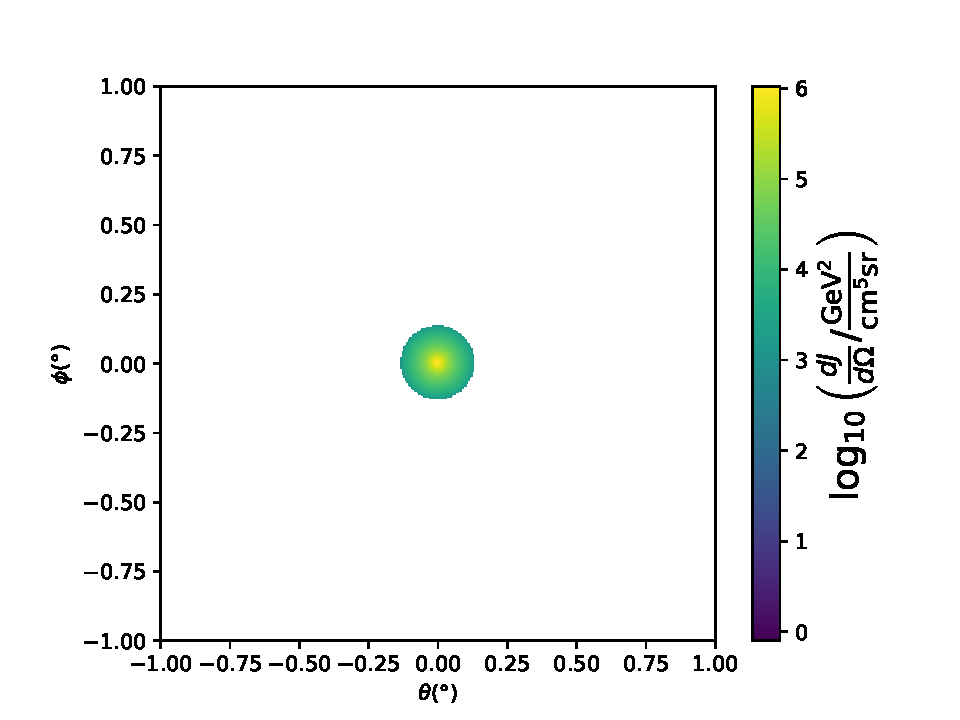
\includegraphics[scale=0.33]{figures/glory_duck/hawc/GD_mass_profiles/LeoIV_J_plot.pdf}
        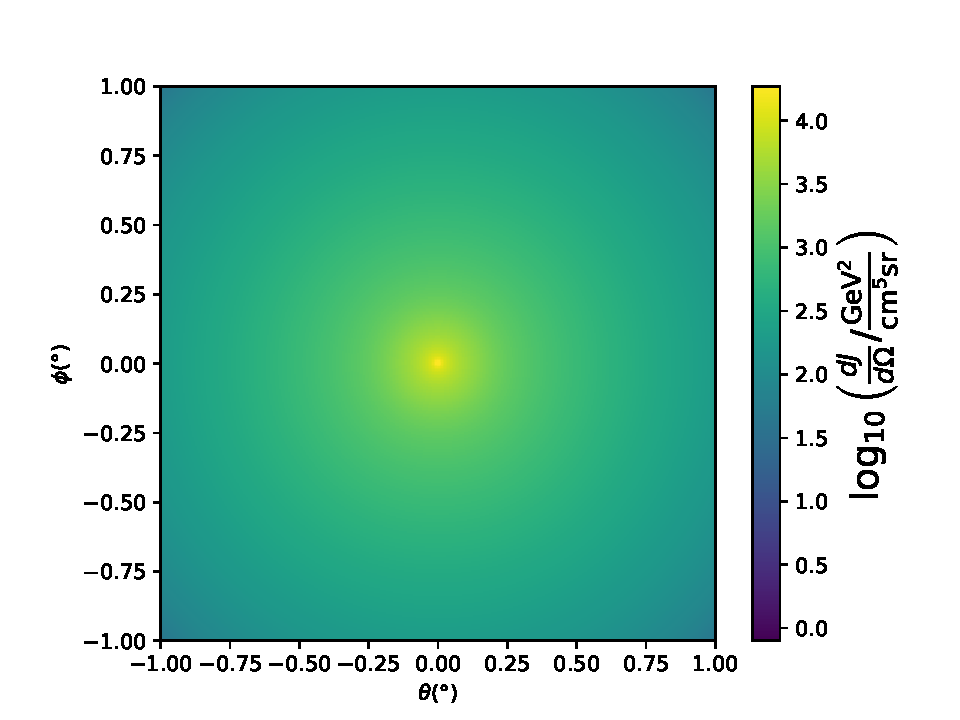
\includegraphics[scale=0.33]{figures/glory_duck/hawc/GD_mass_profiles/Sextans_J_plot.pdf}
        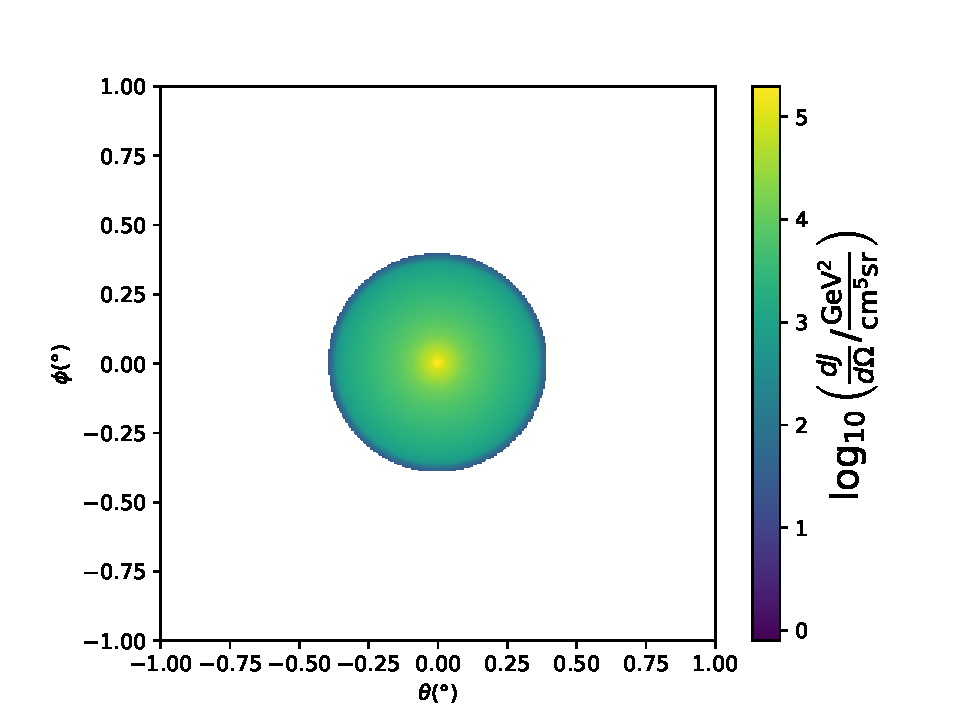
\includegraphics[scale=0.33]{figures/glory_duck/hawc/GD_mass_profiles/UrsaMajorI_J_plot.pdf}
        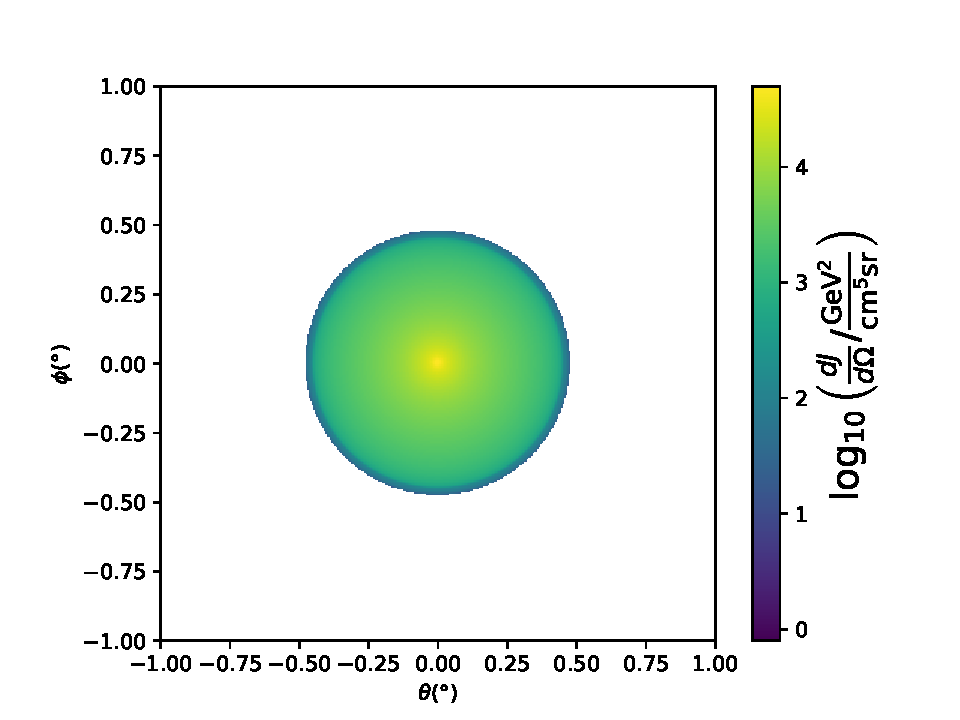
\includegraphics[scale=0.33]{figures/glory_duck/hawc/GD_mass_profiles/UrsaMajorII_J_plot.pdf}
    }
    \caption{Sister figure to \Cref{fig:gd_spatialmodel}. Sources in the first row from left to right: Bootes I, Canes Venatici I, II. In second row: Draco, Hercules, Leo I. In the first row: Leo II, Leo IV, Sextans. In the final row: Ursa Major I, Ursa Major II.} \label{fig:apx_gd_spatialmodels}
\end{figure}